Autonomous drones are an emerging field in both civilian and military sectors. The investment in Zipline, DJI, and other similar companies, show that there is a lucrative market for urban autonomous drone applications such as same-day drone delivery, automated infrastructure inspection, and programmable aerial surveillance~\cite{GrandviewResearchDroneMarket,ForbesZiplineEvaluation}. The rise of companies like Anduril and recent geopolitical events like the War in Ukraine also hint at the wider role that autonomous drones will play in future armed conflicts~\cite{CNBC,CFAS}.

Even with this demand, the quest to make smaller, lightweight autonomous drones is ongoing. Weight scales closely with the capability of onboard compute. Improvements in the artificial intelligence algorithms used for drone perception continue to require more computation to run. This combination of factors makes the prospect of creating a drone system with real-time access to such algorithms challenging.

In this chapter, I provide background on current autonomous drone platforms and outline how some of the obstacles impeding their practical deployment can be overcome. In Section \ref{sec:history-drone-development}, I briefly describe the history of drone development and regulation along with the different categories of modern drones. I also explain the various problems holding these systems back from widespread adoption. In Section \ref{sec:prior-work}, I discuss prior research that has attempted to solve these problems, and its limitations. In Section \ref{sec:better-autonomous-drones}, I propose a possible solution by leveraging the benefits of edge computing and COTS hardware. I show how it addresses the problems facing autonomous drones today and how it improves on previous work.

\section{The Development of Modern Drones}
\label{sec:history-drone-development}

Research into drone technology started in the 1930s when during the interwar period, British engineers created a radio controlled plane, nicknamed the ``Queen Bee'', to train their anti-aircraft gunnery~\cite{IWMDrone}. The Queen Bee's name would spawn the colloquial ``drone'' moniker when referring to radio-controlled aircraft, a reference to worker drones in bee colonies. Over the next several decades, militaries around the world began incorporating drones into their arsenals; first, as pilotless training targets but later, as remotely operated observation and strike aircraft. By the 1990s, drones had become very sophisticated, equipped with multiple onboard sensors which enabled these platforms to conduct aerial reconnaissance at great distances~\cite{GlobalHawk}. Despite these advances, one core design tenet remained unchanged: drones were controlled in every respect by a remote human pilot. Such pilots would be referred to as the remote pilot-in-command (RPIC).

\begin{figure}%
    \centering
    \subfloat[\centering The British-made "Queen Bee", introduced in 1935, was one of the first radio operated aircraft and served as an anti-aircraft practice target~\cite{IWMDrone}.]{{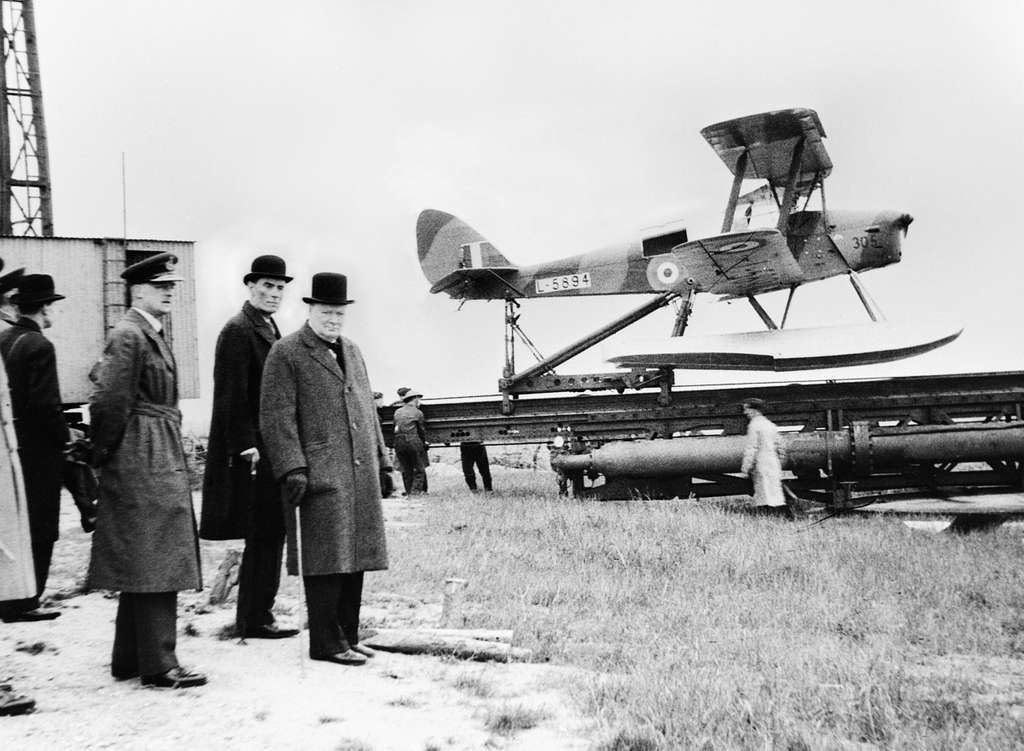
\includegraphics[width=7cm, height=5cm]{chapter2/FIGS/qbee2.jpg}}}%
    \qquad
\subfloat[\centering The RQ-4 Global Hawk, introduced in 1998, is a currently operated US Air Force reconnaissance drone with a range of over 14,000 miles~\cite{GlobalHawk}.]{{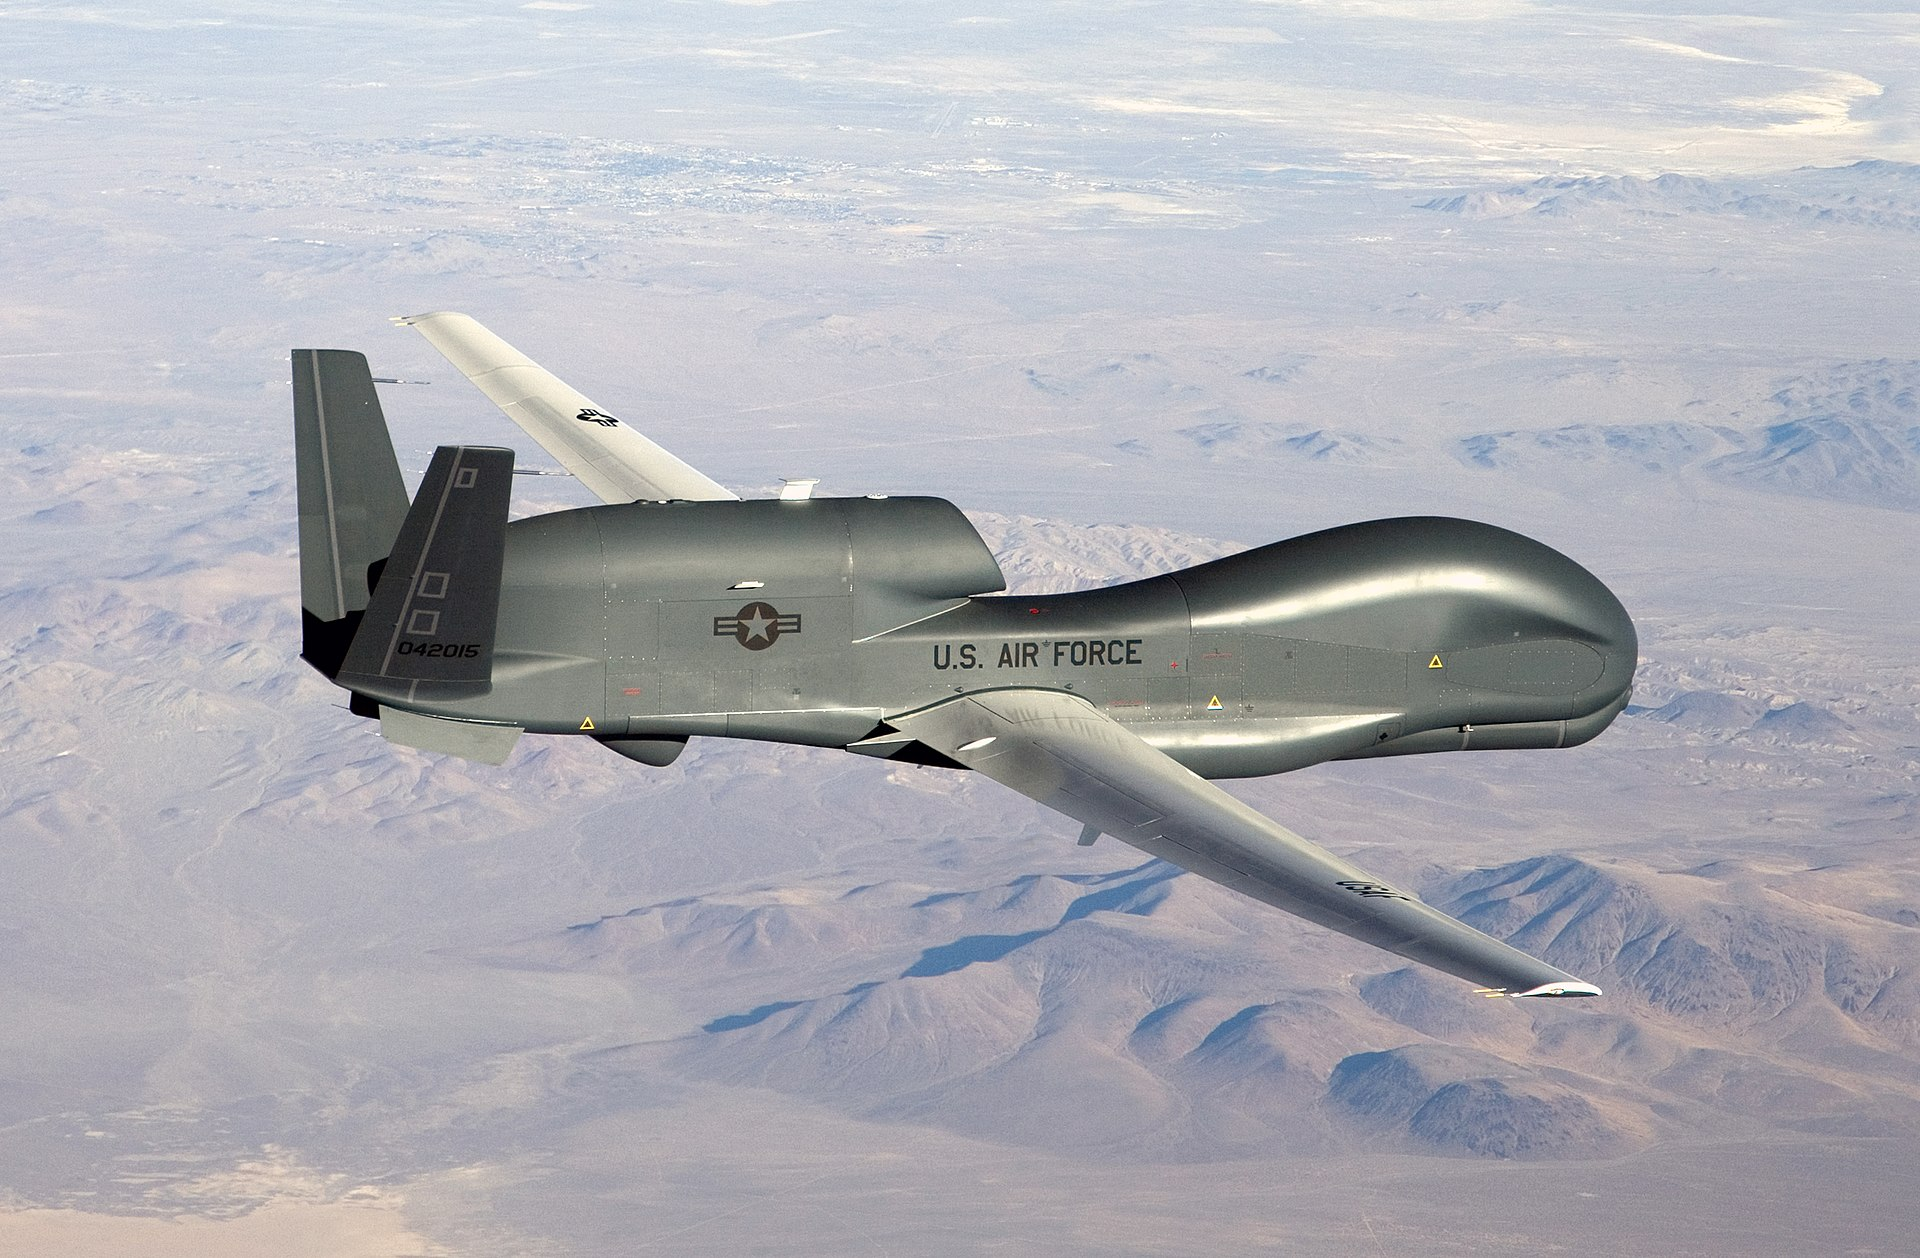
\includegraphics[width=7cm, height=5cm]{chapter2/FIGS/globalhawkdrone.jpg} }}%

    \subfloat[\centering The Skydio 2 platform, released in 2019, provides a small set of semi- and fully-autonomous capabilities like person tracking and obstacle avoidance~\cite{Skydio2,Skydio2Plus}.]{{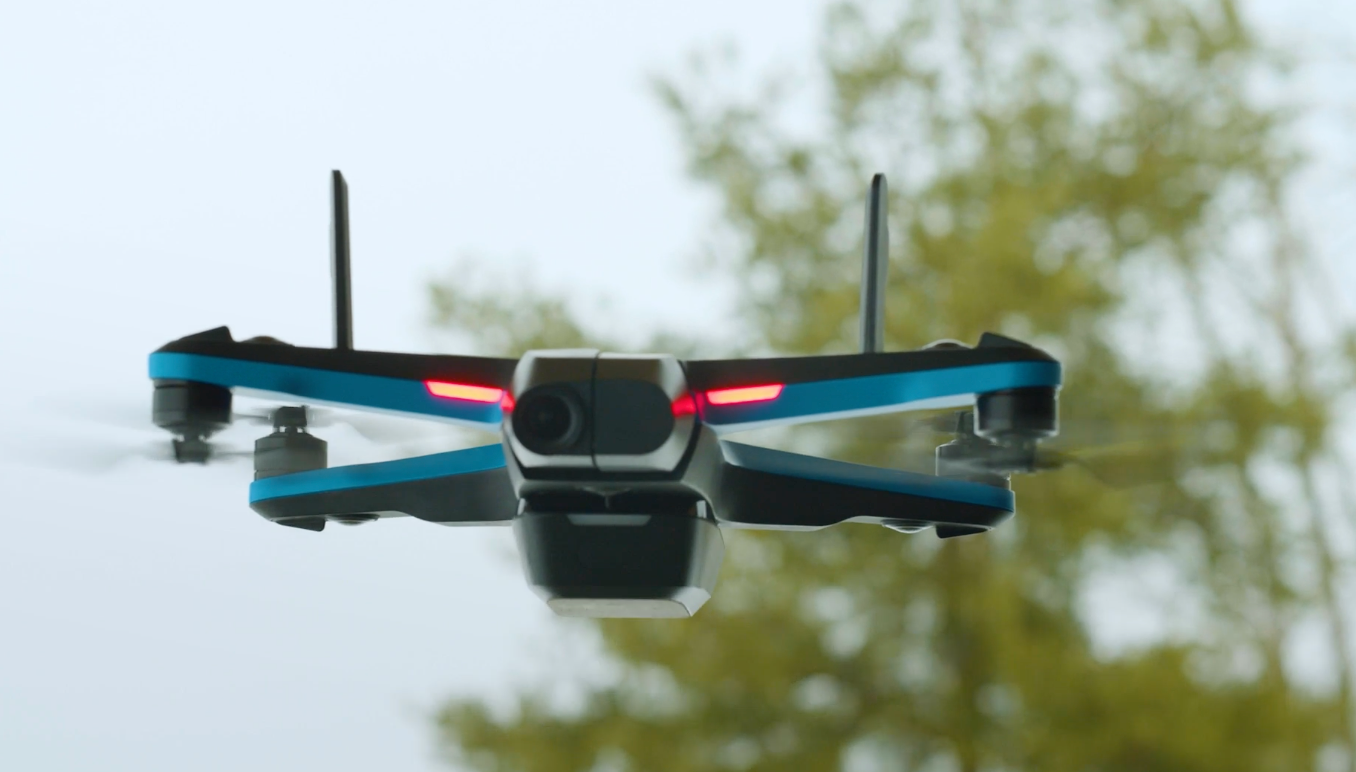
\includegraphics[width=7cm, height=5cm]{chapter2/FIGS/skydio-2.png} }}%
    \qquad
    \subfloat[\centering The DJI Matrice 600, released in 2016, is a fully-programmable autonomous drone with support for native onboard GPUs. Its huge size limits practical deployment~\cite{DJIMatrice}.]{{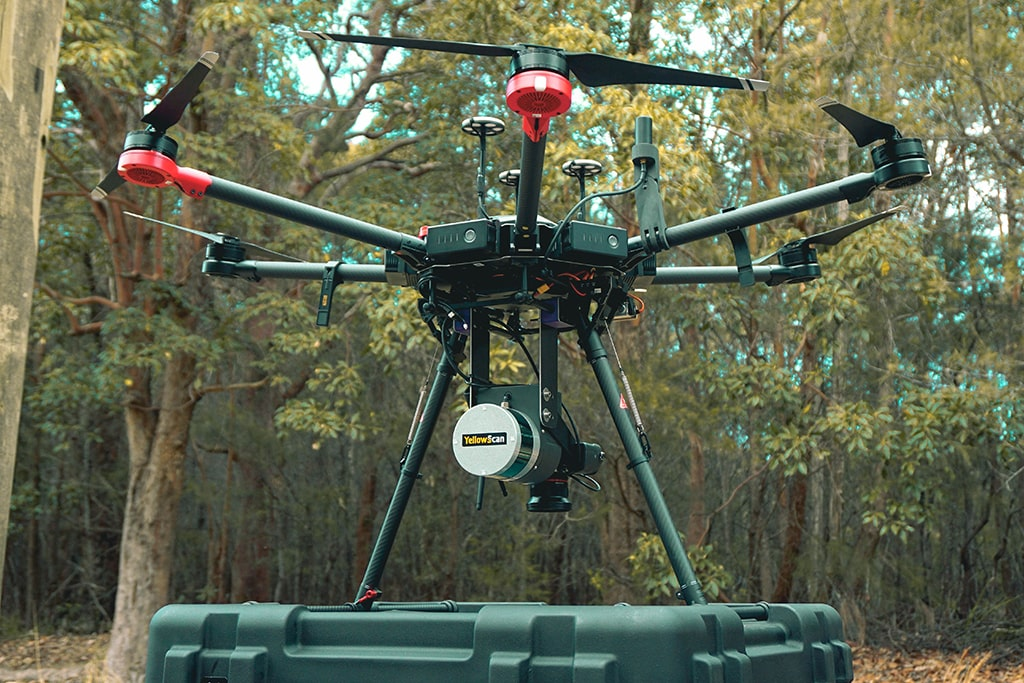
\includegraphics[width=7cm, height=5cm]{chapter2/FIGS/matrice600-2.png} }}%
    \caption{Evolution of Drone Technology}%
    \label{fig:20th-century-drones}%
\end{figure}

In the mid 2010s, drone technology started to shift away from exclusive manual piloting. The release of commercial autopilots (\S\ref{sec:drone-anamtomy}) like PX4 and Ardupilot enabled the rise of miniaturized (under 2~kg) multirotor drones which could perform limited autonomous flight such as following preset GPS waypoints~\cite{PX4,Ardupilot}. Later, this was extended to semi-autonomous visual tracking and autonomous obstacle avoidance in quadrotor offerings like the DJI Phantom 4 and the Skydio 2~\cite{DJIPhantom4,Skydio2}. At the same time, growing investment in commercial fully-autonomous drones yielded the first off-the-shelf products. The DJI Matrice series was the most prominent of these, and it offered fully-autonomous capabilities using an onboard embedded computer, the DJI Manifold~\cite{DJIMatrice}.

While the drone space is diverse in both aircraft size and type, this dissertation will focus on quadrotor drones. Quadrotors are by far the most common drone type and have a number of advantages over fixed-wings and helicopters. Namely, they are affordable, easy to use, and are very stable in multi-directional flight. These make them perfect for tasks involving aerial imagery analysis which are the main focus of this dissertation. For the rest of this document, all mention of ``drones'' will refer to quadrotor aircraft.

\begin{figure}
    \centering
    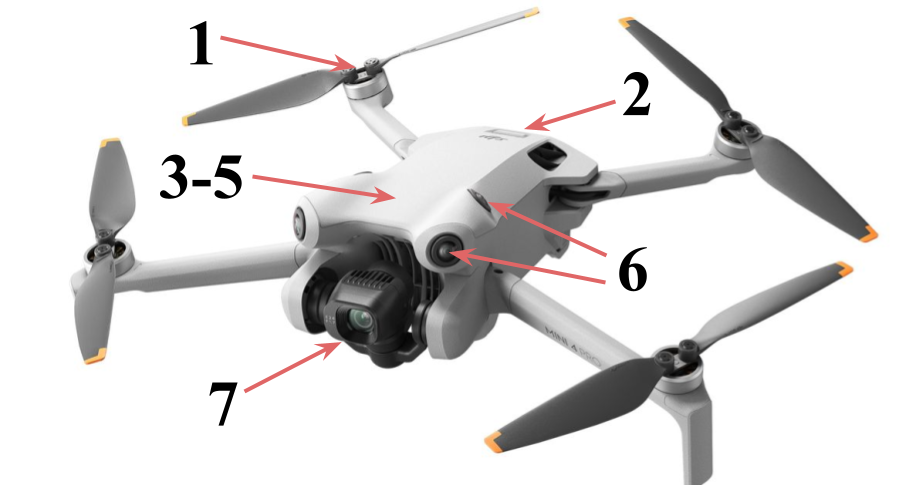
\includegraphics[width=0.75\linewidth]{chapter2/FIGS/anatomy.png}
    \begin{captext}
    \small \\ The main components of a modern consumer drone: \\\textit{\textbf{1.} rotors, \textbf{2.} hot-swappable battery, \textbf{3.} autopilot, \textbf{4.} sensor module, \\ \textbf{5.} companion computer, \textbf{6.} stereo cameras, \textbf{7.} gimbal camera.}
    \end{captext}
    \caption{Quadrotor Drone Anatomy~\cite{DJIMini4}}
    \label{fig:drone-anatomy}
\end{figure}

\subsection{Anatomy of a Drone}
\label{sec:drone-anatomy}
Modern drones are made up of several core components. Broadly, these accomplish one of four tasks: \textit{low-level flight control, high-level flight control, power, and sensing}. Figure~\ref{fig:drone-anatomy} uses the DJI Mini 4 Pro~\cite{DJIMini4}, a popular consumer drone, to illustrate these components:

\begin{enumerate}
    \item \textbf{Rotors} (low-level flight control): provide lift to the aircraft. Opposing pairs counter-rotate to provide stability~\cite{Allain2017}. Rotors are coordinated by the electronic speed controller (ESC), a micro-controller connected to the \textit{Autopilot} module~\cite{Nagel2023}.
    \item \textbf{Battery} (power): delivers power to all components. In many consumer drones, like the DJI Mini 4 Pro, the battery is a separate part which can be easily swapped out in the field.
    \item \textbf{Autopilot} (low-level flight control): works with the ESC to execute flight maneuvers. Uses telemetry from the \textit{Sensor Module} to compensate against the wind and maintain a stable hovering position. Acts as a software abstraction layer over all drone sensors and hardware. Also manages the radio connection to the pilot.
    \item \textbf{Sensor Module} (sensing): provides information about the drone's position and orientation, also known as telemetry. Usually made up of a GPS antenna, an inertial measurement unit (IMU)~\cite{IMU}, an altimeter, and a compass.
    \item \textbf{Companion Computer} (high-level flight control): responsible for high-level autonomous decision-making. Runs computer vision or sensor fusion algorithms, then sends actuation commands to the \textit{Autopilot} based on the outputs.
    \item \textbf{Stereo Cameras} (sensing): gives a real-time depth map of the drone's surroundings~\cite{Stereo}. This enables full 360-degree obstacle avoidance. Not a feature on all consumer drones but becoming increasingly common.
    \item \textbf{Gimbal Camera} (sensing): the main camera through which the drone visually senses its surroundings. Able to pitch, yaw, or roll as commanded by the \textit{Autopilot}.
\end{enumerate}
In some cases, drones may be equipped with special equipment like LIDAR, time-of-flight sensors, RTK modules, and cellular modems. These are rare and are usually a feature of purpose-built aircraft for specific mission sets. 

\begin{figure}
    \centering
    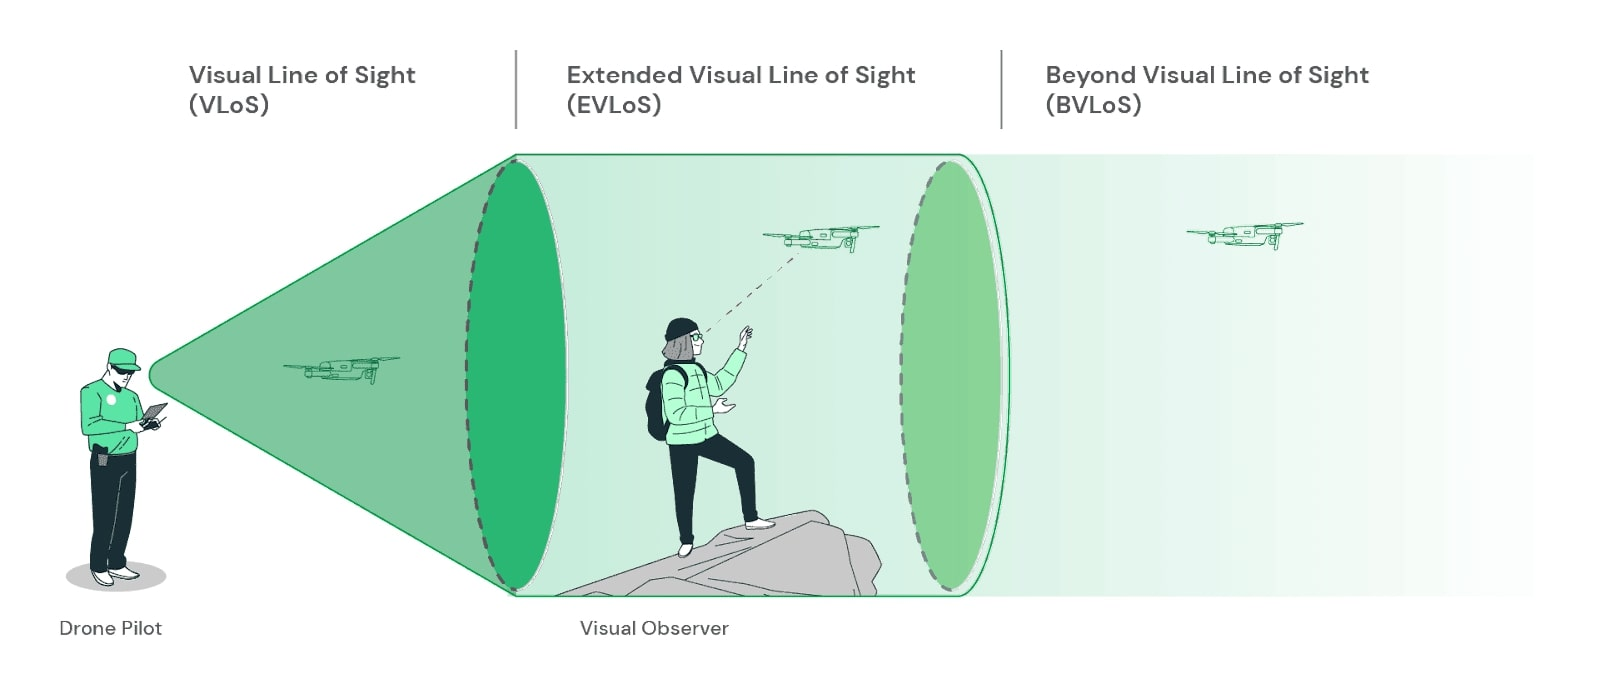
\includegraphics[width=1.0\linewidth]{chapter2/FIGS/bvlos.jpg}
    \caption{Types of Line-of-Sight Operation~\cite{Flytbase}}
    \label{fig:bvlos}
\end{figure}

\subsection{Regulation in Civilian Airspace}
Drones like the DJI Mini 4 Pro and others are available globally for purchase, generally without the need for a license. This has led to a rapid dissemination of drones to consumers across the world and has spurred government regulators into action. This regulation serves one major purpose: to prevent potential damage to people or property due to in-flight emergencies. In the United States, the Federal Aviation Administration (FAA) introduced the Part 107 regulation in 2016~\cite{Flexairco}. This explicitly outlined the classes of UAVs allowed to fly over people, citing that only aircraft under 0.55~lbs or 250~g enjoyed near-unconditional approval~\cite{FAA2021}. In Europe, the European Union Aviation Safety Agency (EASA) has introduced similar regulation, only permitting flights over uninvolved pedestrians for drones under 250~g~\cite{EASA}. Flights over assemblies of people are not allowed for any weight class. In other countries, drones under 250~g are not regulated at all~\cite{IndiaRegulation,ChinaRegulation}.

In addition to weight regulation for flights over people, most countries also have restrictions on beyond visual line-of-sight (BVLOS) operation of heavy drones. Figure~\ref{fig:bvlos} shows the different classes of line-of-sight operations. Visual line-of-sight (VLOS) operation requires the drone pilot to be within direct line-of-sight of the drone. Extended visual line-of-sight (EVLOS) operation permits the pilot to lose visual contact with the drone but requires other human spotters, also known as ``visual observers'' to be within line-of-sight of the drone and in constant radio contact with the pilot. BVLOS operation does not require the pilot or any visual observers to be within line-of-sight of the drone~\cite{BVLOS}. This makes BVLOS flights dangerous; if a collision is imminent, there is no guarantee that the pilot will be notified in time to stop it. Consequently, regulations are stringent for heavier drones due to their greater damage potential.

\subsection{The Current COTS Drone Market}
\label{sec:current-market}
As a result of both regulation and consumer demand, the current commercial-off-the-shelf~\cite{FAR} (COTS) drone market is segmented into three loose categories: fully-autonomous, semi-autonomous, and manually piloted drones. Each of these inhabits a different weight and mission class, and are designed to operate in different regulatory environments. Table~\ref{tab:drone-apps} exhibits the main applications that drones are designed for. Generally, depending on regulation in the mission area, either a semi-autonomous (heavily-regulated) or fully-autonomous (lightly-regulated) drone will be used. 

\begin{enumerate}
    \item \textbf{Manually-Piloted Drones}: Manually-piloted drones are designed for hobbyist consumers, usually for the purpose of drone racing or recreational RC flight. They have no onboard compute, are not programmable, and must be manually piloted at all times to function. An example of a manually-piloted drone is the iFlight Cidora. This class of drone is extremely lightweight and very affordable compared to both semi- and fully-autonomous drones. The iFlight Cidora weighs 115~g and costs \$295 per unit~\cite{Cidora}. Most manually-piloted drones are so light that they avoid regulation. However, they are the least accessible of the three drone classes. This is because they lack any auto-stabilization, and must be flown by an experienced pilot to avoid crashes.
    \item \textbf{Semi-Autonomous Drones}: Semi-autonomous drones have limited onboard compute and cannot perform active vision tasks without a human in the loop. They are typically equipped with a commercial autopilot like PX4 which enables autonomous following of GPS waypoints. They are not intended to operate BVLOS and often require a constant link to the RPIC (remote pilot in command). This is because their main use case is aerial photography and videography. For this reason, this class of drones is commonly referred to as \textit{photography drones}. An example of a photography drone is the Parrot Anafi. It is programmable and has no onboard compute, but can follow GPS waypoints and perform limited visual tracking by utilizing compute resources on the RPIC's remote controller. Photography drones are lightweight and affordable compared to fully-autonomous drones, and can usually be flown in dense urban environments with minimal regulatory hurdles. The Parrot Anafi, for instance, weighs 320~g and costs \$470 per unit~\cite{ParrotAnafi}. They are also the most accessible of the three drone classes since they are designed to be flown by non-pilots and are by far the most widely-used of the three classes. They usually feature excellent stabilization, good safety characteristics, and a simple user experience. 
    \newpage
    \item \textbf{Fully-Autonomous Drones}: Fully-autonomous drones have significant compute resources onboard and are able to analyze their own sensor streams in real time. They can perform active vision tasks without human assistance and can operate BVLOS. They also are fully-programmable, outfitted with an onboard computer and a flight control API. An example of a fully-autonomous drone is the DJI Matrice series. This class of drone is typically heavy and expensive. The Matrice 30, for instance, is over 3.5~kg and over \$10,000 per unit~\cite{Matrice30T}. Because of their size and weight, fully-autonomous drones are generally limited to use in rural areas away from people or property. They are also highly inaccessible, since their large size and complicated user interfaces often require experienced programmers and mission planners to operate safely. 
\end{enumerate}
In reality, most drones share traits from all three of these categories, and seldom fit into one cleanly. This motivates viewing the drone space as a ``spectrum of autonomy''. Typically, this spectrum is segmented into six levels of increasing automation: levels 0-1 corresponding to manually-piloted, levels 2-3 corresponding to semi-autonomous, and levels 4-5 corresponding to fully-autonomous~\cite{Cloudfactory}. This is similar to the levels of automation for self-driving cars~\cite{EPA}. Figure~\ref{fig:spectrum} shows the capabilities of several drones and where they would lie on this spectrum.


\begin{table}
    \centering
    \rowcolors{2}{gray!10}{white}
    \begin{tabularx}{\textwidth}{| m{2.8cm} | m{12.5cm} |}
        \hline
        \centering \makecell{\textbf{*} Precision\\Agriculture} & 
        \small Drones are very useful for precision agriculture, with uses in monitoring, planting, irrigation, and pollination. They are easily scalable for large crop fields and can cover more area than ground-based solutions~\cite{Croptracker}. Most drone agriculture solutions use heavy, fully-autonomous platforms since rural areas have less strict regulation. \\[0.1cm]
        \hline
        \centering\makecell{\textbf{*} Search and\\Rescue} & 
        \small Aerial vehicles have historically been a vital component in search and rescue. Drones fit nicely into this role, allowing search and rescue teams to scan an area at a much lower altitude than they could with traditional aircraft. They have seen real world use in the wake of the 2010 Haiti earthquake and other natural disasters~\cite{SARDrone}. \\[0.1cm]
        \hline
        \centering\makecell{Package\\Delivery} &
        \small For many years, drones have been touted as the future of last mile package delivery. This is because they can operate with higher cost-efficiency for small size items and can reach areas that are not well-connected by traditional infrastructure~\cite{PackageDrone}. Amazon has invested heavily in Prime Air, a drone-based extension to its popular Prime delivery service. However, this project has been sidelined by FAA regulation~\cite{Link2023}. Other companies like Zipline have had more success, using drones to make 1 million deliveries to remote areas~\cite{ForbesZiplineDeliveries}. \\[0.1cm]
        \hline
        \centering\makecell{\textbf{*} Structure\\Inspection} &
        \small Recently, drones have emerged as a useful tool for structure inspection. They are able to reach inaccessible sections of structures due to their small size and maneuverability. More importantly, they are much safer and efficient than a human inspector. In 2022, the U.S. Bureau of Labor Statistics estimated that 1 in every 5 construction workplace deaths was due to falls~\cite{ConstructionFalls}. Drones allow pilots to view unsafe areas with no personal risk. This has increased the frequency of building inspection checkups, ensuring prompt, safe maintenance on failing infrastructure~\cite{InfrastructureInspection}. \\[0.1cm]
        \hline
        \centering\makecell{\textbf{*} Aerial\\Surveys} &
        \small While aerial surveys and 3D scans have been conducted for decades, drones are a new, more cost effective tool for this task~\cite{AerialPhotography}. Their ability to provide a high resolution, bird's eye view of an area combined with their flight stability, make them ideal candidates for survey work. \\[0.1cm]
        \hline
        \centering\makecell{\textbf{*} Aerial\\Reconnaissance} &
        \small Modern drones have revolutionized police and military aerial reconnaissance. Their small size allows them to be easily carried to mission areas and deployed on-the-fly when necessary~\cite{StarsStripes}. Both U.S. police and military forces have heavily invested in such platforms~\cite{StarsStripes,PoliceDrone}.  \\[0.1cm]
        \hline
        \centering\makecell{Suicide\\Aircraft} & 
        \small Suicide drones have been one of the most impactful new weapons in the War in Ukraine. Both Russian and Ukrainian forces have used small quadcopters like the DJI Mavic 3 to deliver bomb payloads~\cite{BBCKamikaze}. These have been very effective against slow moving targets like tanks~\cite{FPKamikaze}. Some fear that this technology could lead to a new breed of terrorist attacks~\cite{Pledger2021}. \\[0.1cm]
        \hline
        \centering\makecell{\textbf{*} Anti-Drone\\Defense} &
        \small As the threat of drones has increased, the investment in drone defense systems has surged. Companies like Anduril have tackled this problem by using specialized drones to take down other hostile drones. Their Anvil kinetic interceptor destroys other UAVs by smashing into them at high speeds~\cite{Anvil}. \\[0.1cm]
        \hline
    \end{tabularx}
    \\[0.2cm]
    \begin{captext}
        \small
        \textbf{*} These tasks are within the scope of this work since they do not require additional payload.
    \end{captext}
    \caption{Drone Applications}
    \label{tab:drone-apps}
\end{table}

\begin{figure}[]
    \centering
    \begin{tabular}{|c|c|c|c|c|c|c|}
        \hline
           \rowcolor{lightgray!50}
         \textbf{Drone} & \textbf{Autopilot} & \textbf{Avoidance} & \textbf{Tracking} & \textbf{Programmable} & \textbf{Compute} & \textbf{Weight} \\
         \hline
         iFlight Cidora & \cellcolor{green!20}None & \cellcolor{green!20}None & \cellcolor{green!20}None & \cellcolor{green!20}No & \cellcolor{green!20}None & 115~g \\[0.1cm]
         \hline
         DJI Avata 2 & \cellcolor{red!20}Yes & \cellcolor{yellow!20}Partial & \cellcolor{green!20}None & \cellcolor{green!20}No & \cellcolor{green!20}None & 377~g \\[0.1cm]
         \hline
         Parrot Anafi & \cellcolor{red!20}Yes & \cellcolor{green!20}None & \cellcolor{yellow!20}Assisted & \cellcolor{red!20}Yes & \cellcolor{green!20}None & 320~g \\[0.1cm]
         \hline
         DJI Mini 4 Pro & \cellcolor{red!20}Yes & \cellcolor{red!20}Yes & \cellcolor{yellow!20}Assisted & \cellcolor{yellow!20}Partially & \cellcolor{green!20}None & 249~g \\[0.1cm]
         \hline
         Skydio X10 & \cellcolor{red!20}Yes & \cellcolor{red!20}Yes & \cellcolor{red!20}Yes & \cellcolor{yellow!20}Partially & \cellcolor{red!20}Yes & 2110~g \\[0.1cm]
         \hline
         DJI Matrice 30 & \cellcolor{red!20}Yes & \cellcolor{red!20}Yes & \cellcolor{red!20}Yes & \cellcolor{red!20}Yes & \cellcolor{red!20}Yes & 3770~g \\[0.1cm]
         \hline
    \end{tabular}
    \\[0.2cm]
    \begin{captext}
        \small Capabilities are colored according to whether they are typically associated with manually-piloted (green), semi-autonomous (yellow), or fully-autonomous (red) drones.
    \end{captext}
    \\[0.6cm]
    \centering
    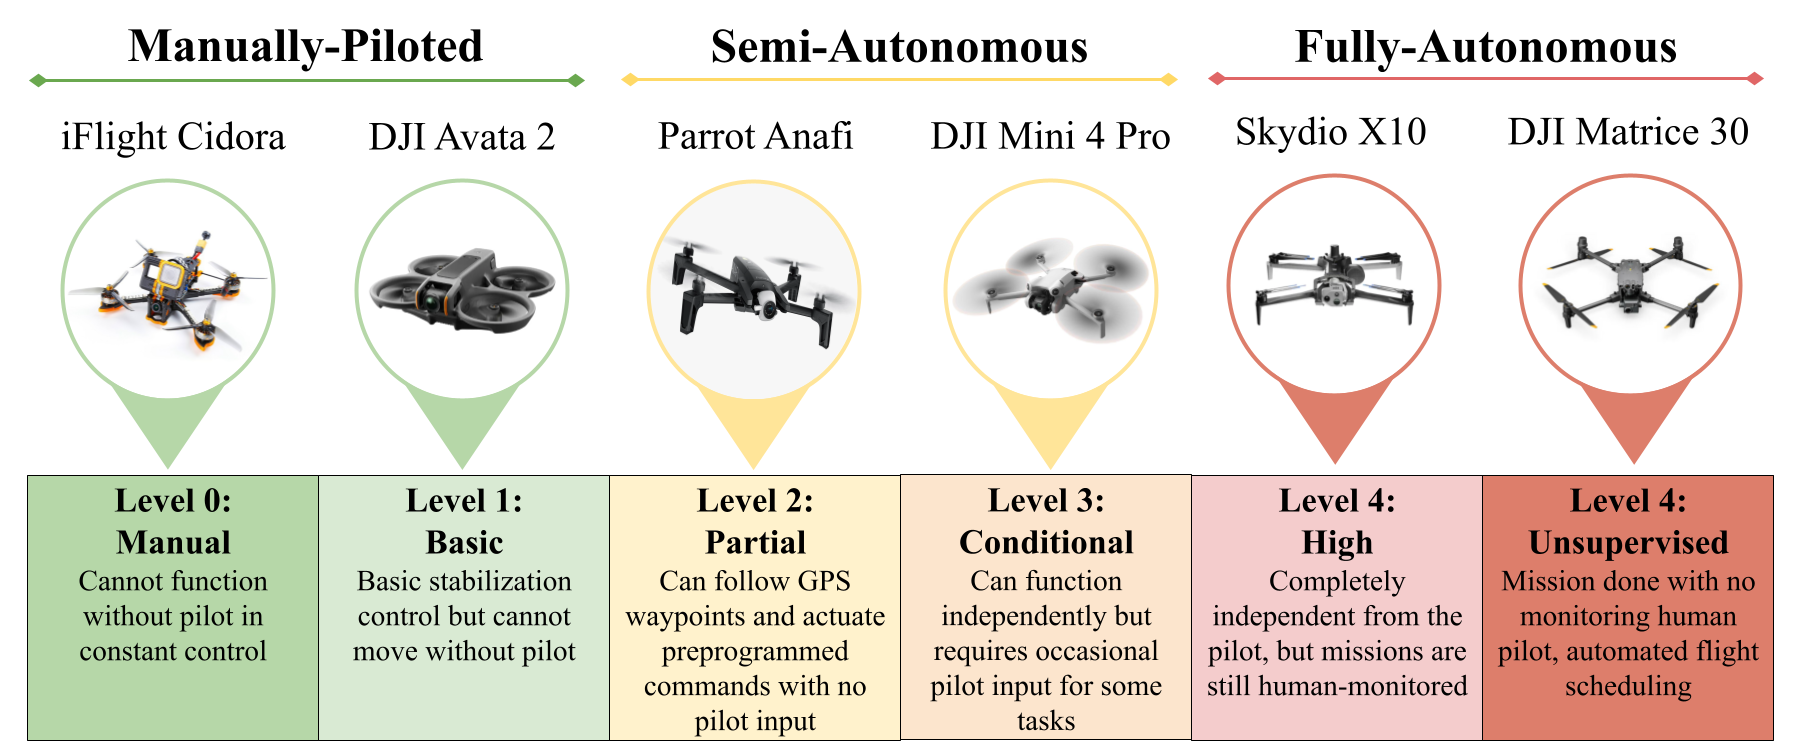
\includegraphics[width=1.0\linewidth]{chapter2/FIGS/spectrum.png}
    \begin{captext}
        \small Based on their capabilities, I have placed each drone on the spectrum of autonomy, broken down by level~\cite{Cloudfactory}. This placement is entirely subjective, but it gives some reference for the differing levels of automation between commercial drone offerings.
    \end{captext}
    \caption{The Spectrum of Autonomy~\cite{Cidora,DJIAvata2,ParrotAnafi,DJIMini4,SkydioX10,Matrice30T}}
    \label{fig:spectrum}
\end{figure}

\subsection{What is Holding Drones Back?}
\label{sec:problems}
As presented by Table~\ref{tab:drone-apps}, there are many applications where drones have been useful. Yet it is my belief that they still have not lived up to their true potential. Many of the listed tasks, such as aerial surveys, building inspection, and police surveillance, are still done using full manual or human-assisted control in densely populated areas. Yet many if not all of these tasks could benefit greatly from full-autonomy, especially in or around cities. Surveys or inspection flights could be performed daily, without human supervision, with an auto-generated report sent out for engineers to look over. This could greatly reduce costs and prevent critical infrastructure failures, potentially saving lives~\cite{Dorafshan2018}. Automated police surveillance could free up officers, reduce training overhead, and provide round-the-clock monitoring without any risk of fatigue. So why have fully-autonomous platforms failed to see widespread use in these urban applications, when they have been used with great success elsewhere?

The answer is complicated, but I believe that there are five clear problems facing fully-autonomous drones in dense urban settings:
\begin{itemize}
    \item \textbf{Weight}: fully-autonomous aircraft are heavy, as discussed in Section~\ref{sec:current-market}. This is because they require onboard compute like GPUs to operate which drive up weight. This directly clashes with most international drone regulation which becomes progressively more restrictive over 250~g.
    \item \textbf{Accessibility}: fully-autonomous drones, due to their size and weight, require experienced pilots to operate safely. They demand careful flight planning and program verification before flight, since a loss of aircraft could be hazardous to people and property. This restricts fully-autonomous drones to a small user-base.
    \item \textbf{Versatility}: there is a major trade-off in current fully-autonomous drone products between weight and versatility. Heavy platforms which carry generalized compute hardware like CPUs and GPUs are versatile since they can run most kinds of software natively. On the other hand, lightweight platforms cannot carry generalized compute due to weight constraints, and thus usually carry specialized compute for only one or two mission types.
    \item \textbf{Portability}: drone manufacturers have their own, tightly integrated software stack that does not work with other drone models. This all-or-nothing approach means that a consumer must stick within the hardware ecosystem or be forced to buy an entirely new fleet of drones.
    \item \textbf{Cost}: fully-autonomous drones typically cost around ten times the cost of comparable semi-autonomous drones. This makes them much less economically viable at scale. 
\end{itemize}
If a commercial product were to solve these five challenges, it is my belief that autonomous drones would see widespread use, even in dense urban environments. At the time of writing this document, no such product exists.

\section{Prior Research}
\label{sec:prior-work}
In parallel to commercial efforts, autonomous drone research has surged in recent years. Real-time execution of active vision tasks has been a key driver. Schedl et al proposed an autonomous drone design for classification-driven adaptive search and rescue in densely forested environments~\cite{Schedl2021}. George et al demonstrated a drone inspection system which could localize the drone's camera view onto a 3D model of a target structure in real time~\cite{George2019}. Chen et al showed an efficient drone onboard computation model for visual object tracking~\cite{Chen2018}. Many other projects have explored similar applications in surveillance, wildlife monitoring, and racing~\cite{Apvrille2014,Li2020,Devos2018,Alsalam2017,Ward2016}.  

A growing number of researchers have identified some of the problems outlined in Section~\ref{sec:problems} (\textit{weight}, \textit{accessibility}, \textit{versatility}, \textit{portability}, and \textit{cost}) as important research areas. In this section, I will present projects that attempt to solve these problems. I will also discuss their limitations and why their solutions have not fully addressed the issues I outlined.


\subsection{Weight}
Since as early as 2009, the drone research community has recognized the importance of lightweight aircraft in real world applications~\cite{Burkle2011, Burkle2009}. Lightweight ($\leq 450$~g) autonomous drones have many benefits over their heavier counterparts: they are safer to operate, have simpler transportation logistics, and have a lower noise profile. It was theorized that achieving such lightweight autonomy would enable the vision of cooperative drone swarms~\cite{Floreano2015}. Since the mid 2010s, much work has focused on bringing high-level autonomy to small, lightweight drones. Schmid et al proposed a sub-1~kg aircraft design which could perform unassisted visual navigation~\cite{Schmid2014}. Palossi et al developed visual navigation and human pose estimation software which runs onboard 27~g drones~\cite{Palossi2019,Palossi2021}. M{\"u}ller et al demonstrated a depth-based obstacle avoidance system for 35~g drones~\cite{Muller2023}. Many of these projects suffer from similar issues of portability; they either use purpose-built aircraft or function on only one type of aircraft. There is little ability to deploy these systems to different drone hardware, a drawback in an ever-changing drone landscape. 

\subsection{Accessibility}
\label{sec:development-platforms}
In the current drone research space, accessibility is not a first-order consideration. Many projects use custom-built aircraft with no guidance on how to replicate the platform for other researchers. In some cases, these custom drones require low-level electrical engineering experience to ensure safe and stable operation. On the other hand, there has been some effort to increase accessibility for drone programming. Beseda et al presented a mission-oriented control infrastructure for easily managing swarms of autonomous UAVs~\cite{Besada2019}. Mottola et al proposed a simple but expressive API for drone team control~\cite{Mottola2014}. Tilley et al developed a block programming language that could allow children to program autonomous drones~\cite{Tilley2017}. While this work is useful, these projects do not present a practical integration strategy with real consumer drones, nor do they circumvent the difficulties of custom-built research platforms.

\subsection{Versatility}
Mission versatility is a feature that most heavy fully-autonomous drones already possess, since they carry generalized compute like CPUs and GPUs which can run GPLs (general-purpose programming languages) and inference deep neural networks with relatively low latency. Achieving this versatility on lightweight drones is an enduring challenge. This is because miniaturizing generalized compute hardware is difficult, and weight-optimized compute hardware is inflexible~\cite{Hu2022}. Still, many have tried to modify lightweight onboard hardware to be able to run heavyweight computer vision algorithms. Albanese et al propose a neural accelerator modification to a Raspberry Pi which could be flown onboard small UAVs~\cite{Albanese2022}. Zhang et al demonstrate an FPGA architecture for drones that can inference neural networks with much lower power demand than GPUs~\cite{Zhang2022}. None of these projects have gained much traction, likely due to their poor practicality and usability.

Corporate research projects have yielded promising results, such as the ModalAI Starling series and the Bitcraze Crazyflie shown in Figure~\ref{fig:drone-dev-platforms}. These both use custom compute hardware to provide a Linux programming environment in an ultra-lightweight package~\cite{Bitcraze, ModalAI}. Still, these systems do not truly capture the versatility of CPU/GPU-based systems, and neither fully support the open-source libraries which drive most computer vision research, like OpenCV and PyTorch. This significantly hinders practical use.

\begin{figure}
    \centering
    \subfloat[\centering Bitcraze Crazyflie~\cite{Bitcraze}\\(27~g)]
    {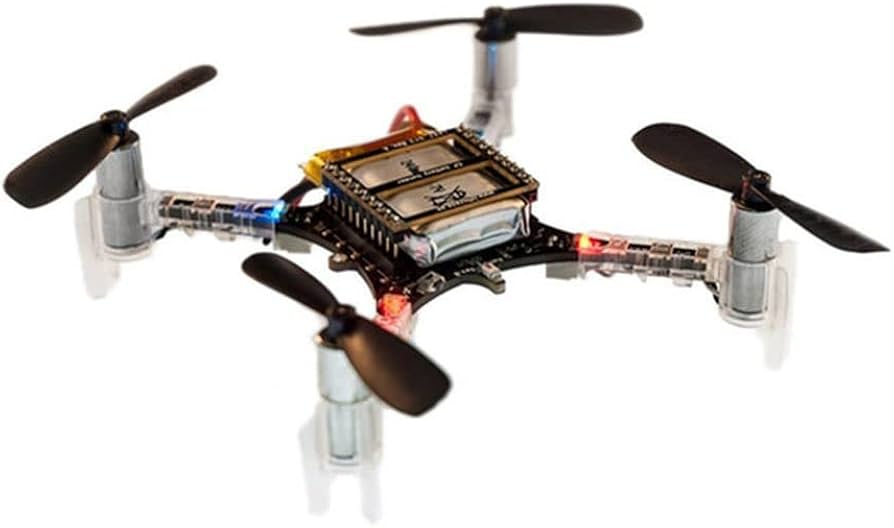
\includegraphics[width=0.30\textwidth, height=1.5in]{chapter2/FIGS/crazyflie.jpg}}
    \qquad
    \subfloat[\centering Modal AI Starling~\cite{ModalAI}\\(280~g)]
    {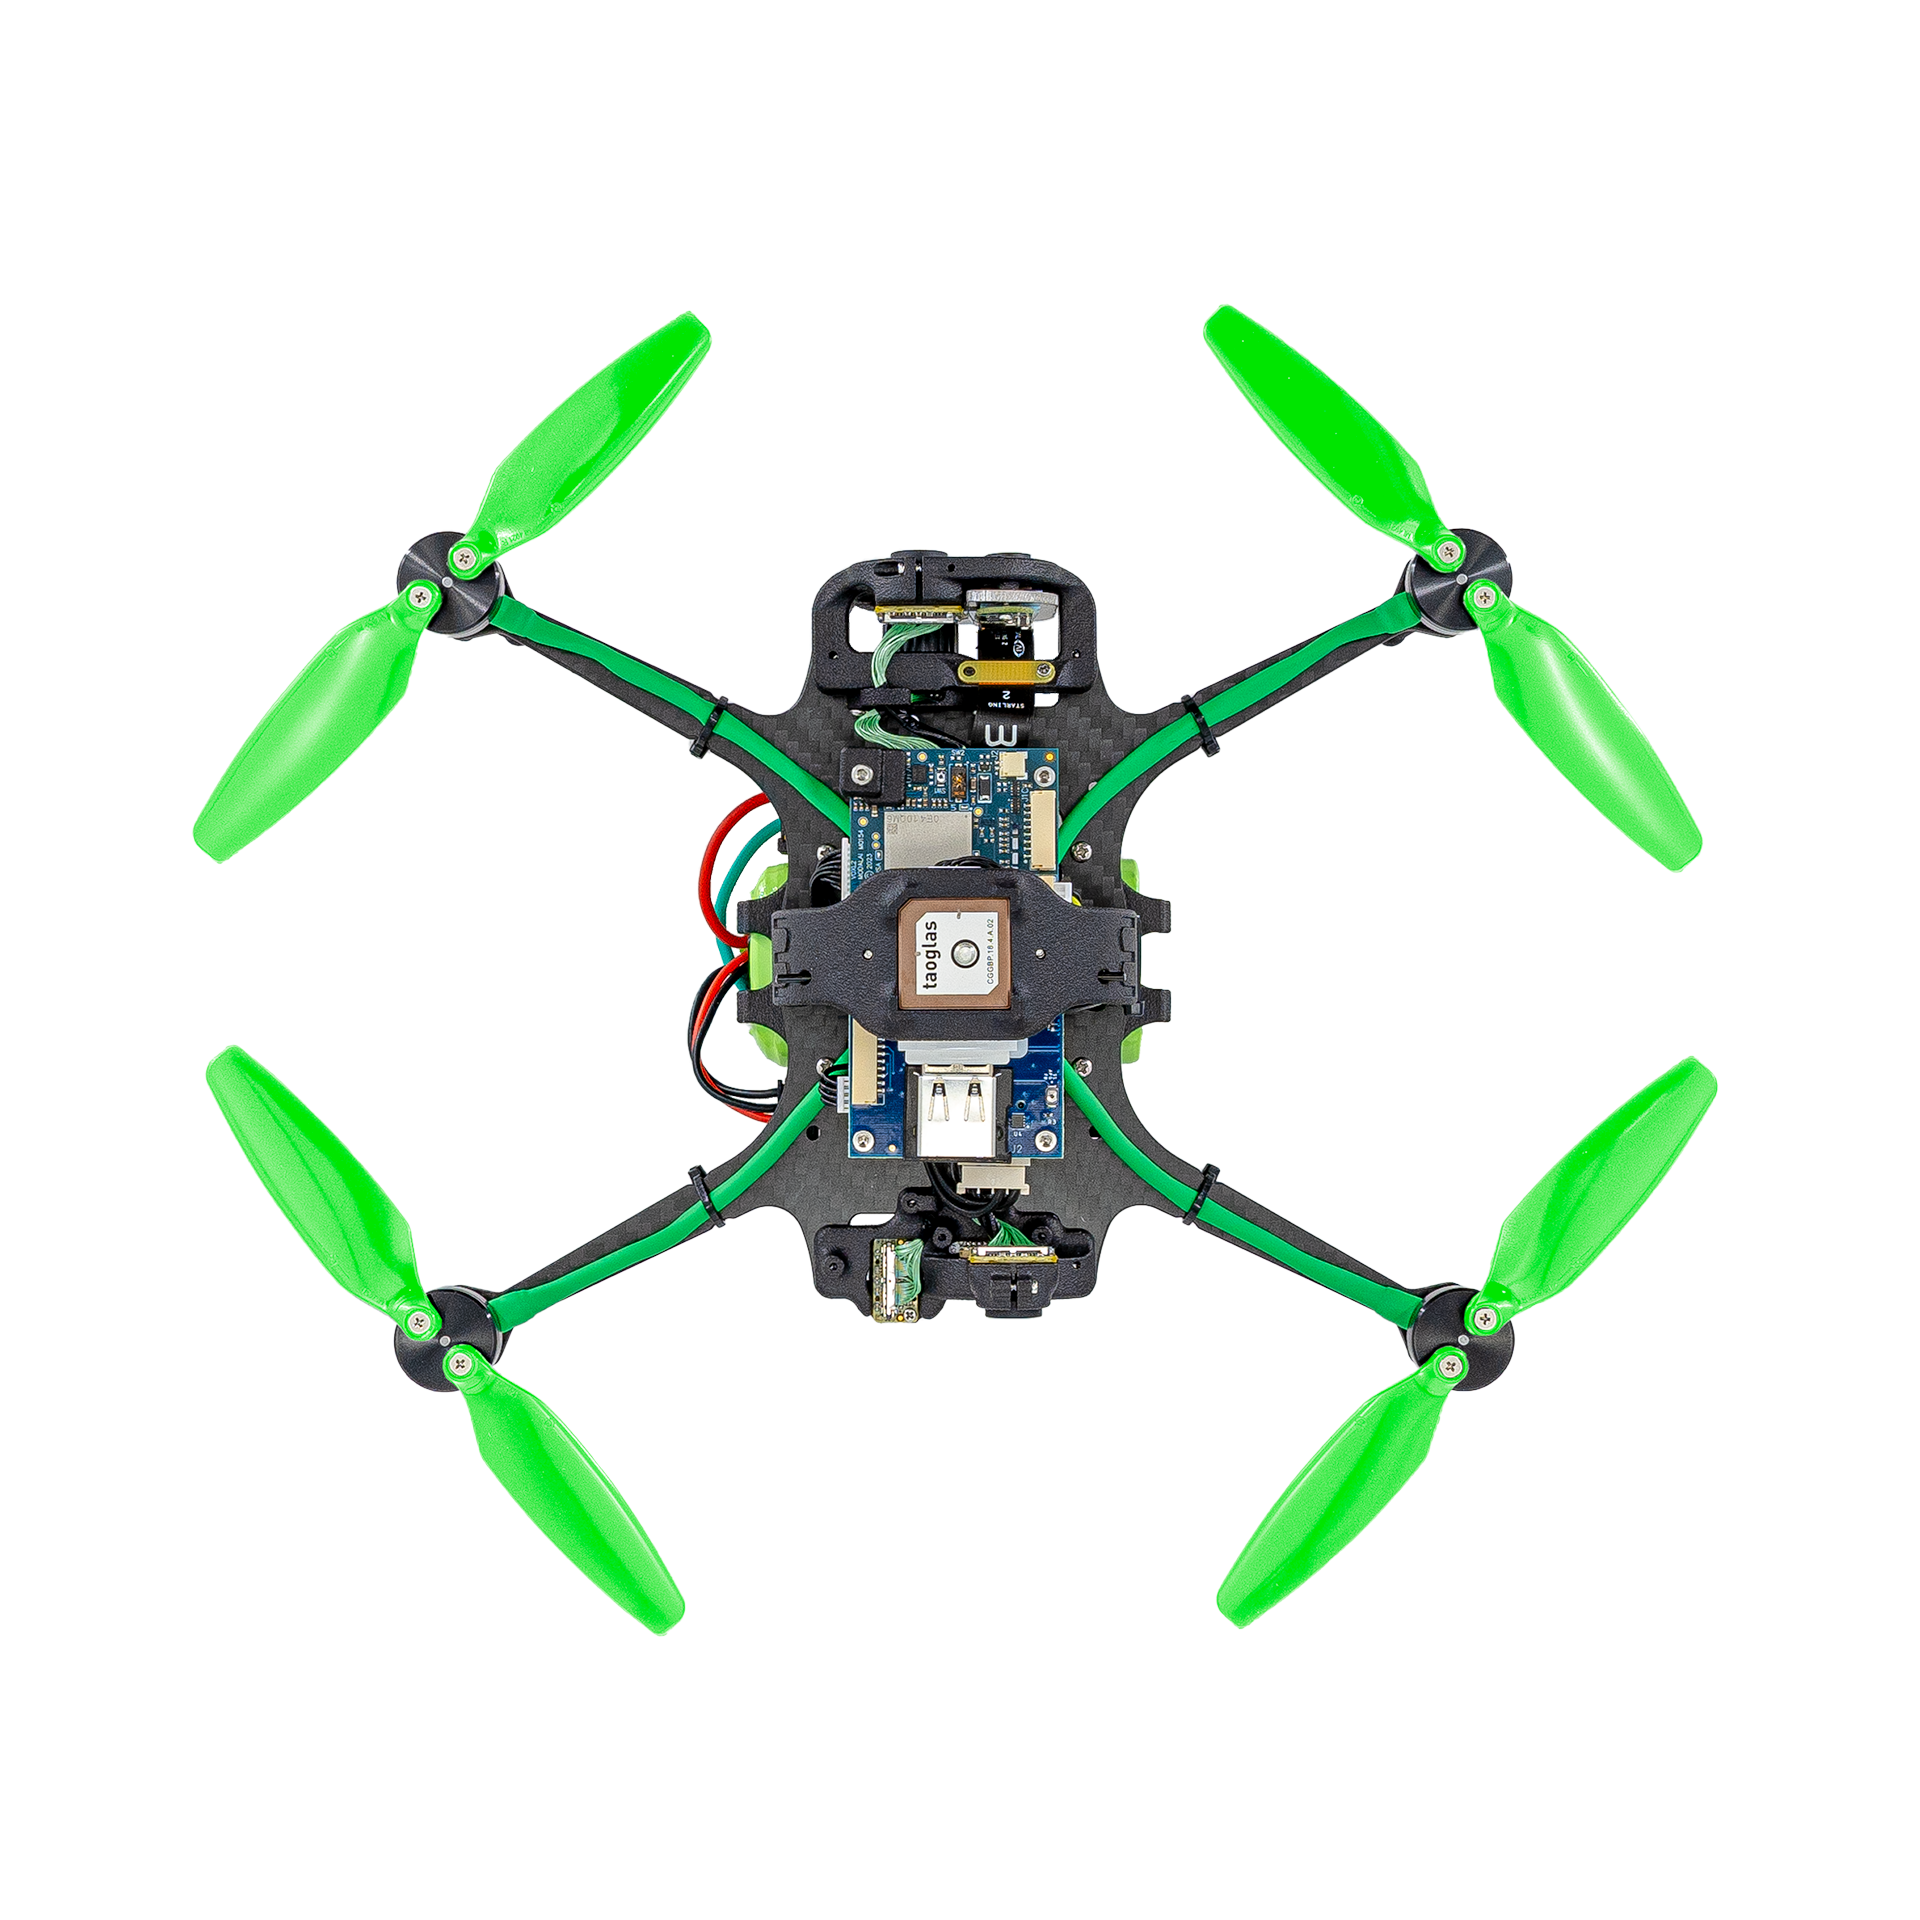
\includegraphics[width=0.30\textwidth, height=1.75in]{chapter2/FIGS/starling-2.png}}
    \caption{Consumer Drone Development Platforms}
    \label{fig:drone-dev-platforms}
\end{figure}

\subsection{Portability}
The ability to seamlessly switch underlying drone hardware has only recently become a hot research topic. This is motivated by greater research impact; cross-platform drone work has a much wider reach. One example of such work is BeeCluster, a drone-agnostic swarm orchestration tool with a simplified task programming interface~\cite{He2020}. BeeCluster supports drones that talk using the BeeCluster protocol, and provides a high-level API wrapper over this protocol. As of the time of writing this document, no guidance has been provided by the authors on how to integrate a new drone platform into BeeCluster, but the framework theoretically allows for heterogeneous swarm operation~\cite{BeeCluster}.

\subsection{Cost}
Driving down cost has been an enduring goal of the drone research community. Eller et al designed a low-cost autonomous platform for under \$225~\cite{Eller2019}. Hardy et al used a sub-\$1,000 drone to map malaria breeding grounds~\cite{Hardy2017}. S{\o}rensen et al proposed an \$800 aircraft for mobile remote sensing~\cite{Sorensen2017}. Projects like these aim to make drones more economically viable, especially in regions with less purchasing power. However, none are concerned with the other important challenges outlined, like weight.  

\section{Towards Better Autonomous Drones}
\label{sec:better-autonomous-drones}
The key factors of \textit{weight}, \textit{accessibility}, \textit{versatility}, \textit{portability}, and \textit{cost} all hinder autonomous drone development and deployment, yet no proposed system has solved all of these issues simultaneously. Clearly, significant research effort has been spent on solving these problems; so why does no such system exist? Central to the answer is what I call the \textit{onboard compute trade-off}. The onboard compute trade-off is a property of unmanned aerial platforms that claims:

\begin{displayquote}
Traditional hardware, like CPUs and GPUs, offers the benefit of versatile, software portable, cost-effective compute power at the expense of weight. Specialized hardware offers the benefit of light weight at the expense of versatile, software portable, cost-effective compute power. Thus, in order to reduce weight, \textit{versatility, portability, and cost must be compromised}.
\end{displayquote}

This fact has limited the development of lightweight fully-autonomous drones and it is chiefly responsible for the gap that exists in the drone market today. Unfortunately, even with recent technological advances, it is unclear whether this challenge can be solved. But, there may be ways it can be circumvented.

\subsection{The Advent of Edge Computing}
Over the past few years, a new computational paradigm has emerged called \textit{edge computing}. Edge computing gives mobile devices access to strong computational resources at low latency by offloading to a network-proximal server~\cite{Satya2017}. In many ways, this is similar to cloud computing. The theory is that mobile devices will always be resource-poor compared to data centers. By sending compute jobs over the network, running on the vast compute of a data center, and getting the result back, mobile devices can mitigate their computational deficiencies. 

The insight of edge computing is that some computation is \textit{latency-sensitive}. That is, the faster the result is returned to the user, the better the system performs. This is usually the case for interactive applications, like augmented reality, or for reactive applications, like robotic actuation in response to visual stimuli. In these cases, sending a compute job to the cloud may be too slow. Edge computing positions smaller groups of servers, called cloudlets, physically closer to mobile clients, usually co-located with cell towers. This hugely decreases latency without sacrificing much per-user compute power, since cloudlets, due to their smaller reach, have fewer tenants than cloud servers~\cite{Charyyev2020,Dolui2017}.

\begin{figure}
    \centering
    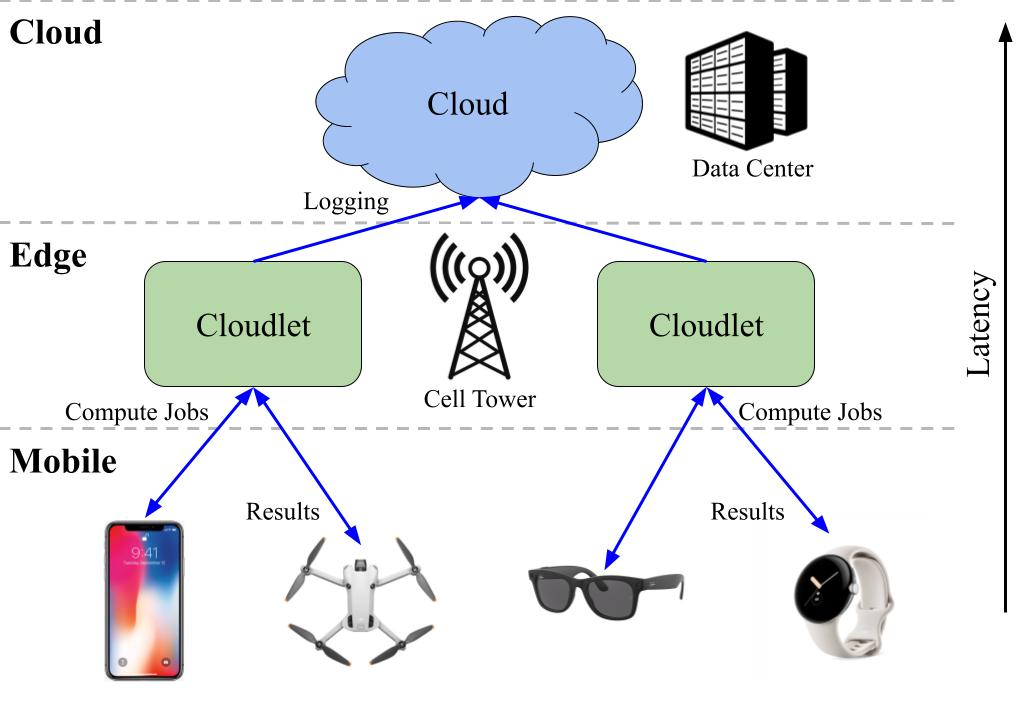
\includegraphics[width=0.9\linewidth]{chapter2/FIGS/edge-computing.jpg}
    \caption{Edge Computing Paradigm}
    \label{fig:edge-computing}
\end{figure}

\subsection{Autonomous Drones and the Edge}
\label{sec:drone-and-the-edge}
Edge computing offers a compelling alternative to the onboard compute trade-off. Instead of miniaturizing compute to fly with a drone, it is much easier to relocate heavyweight compute to the edge so that it is accessible with low latency. This has a number of important advantages over traditional onboard computation paradigms:

\begin{itemize}
    \item The underlying hardware where compute runs is well-understood and general purpose (server-grade CPUs and GPUs). This hugely increases portability and offers a developer-friendly programming environment.
    \item The cost of edge-enabled drones is low; there is no longer a need for expensive lightweight compute hardware, only a relatively cheap modem to communicate with the edge. This greatly increases scalability and thus the economic viability of drone swarms.
    \item Server-grade compute power will always vastly exceed mobile compute power~\cite{Qi2012}. This opens the door to real-time inference of heavy models like transformers.
\end{itemize}

An edge computing approach is not without its drawbacks. The drone is now fully reliant on its communication link with the cloudlet, meaning it is susceptible to service disruptions and bandwidth constraints. This is no worse than manually-piloted drones, which are also dependent on a communication link to the RPIC. Still, these factors must be accounted for in any successful edge-based drone system.

Edge-enabled drones are not a new idea. For several years, researchers at the intersection of edge computing and robotics have published many influential papers on the topic~\cite{Wang2017,Bertizzolo2020,Asaamoning2021,Gharibi2016}. In
these projects, drones use a ground station or cloudlet in conjunction with other nearby aircraft to offload high compute loads. However, this previous work either focused on the theory of how such a system should be designed or on solutions using custom components. None identified weight as a major constraint, and so they failed to present a practical, fully-functional system for public flight operations.

\begin{figure}
    \centering
    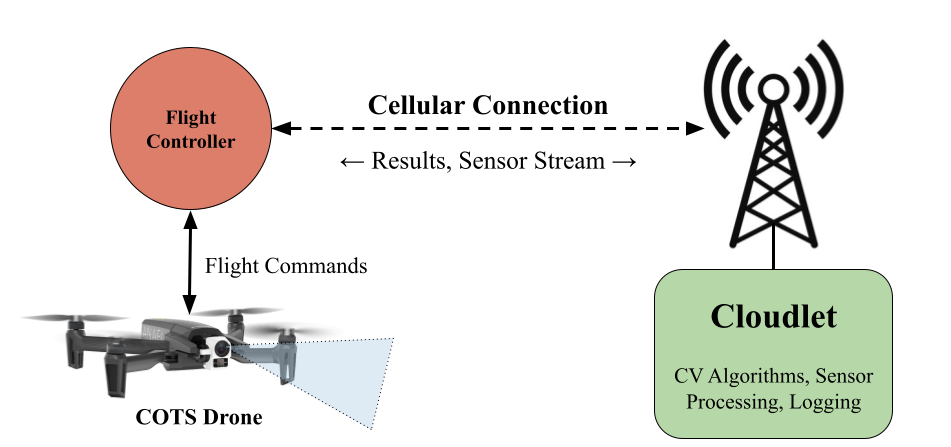
\includegraphics[width=1.0\linewidth]{chapter2/FIGS/simplearch.png}
    \caption{SteelEagle Autonomy Model}
    \label{fig:steeleagle-model}
\end{figure}

\subsection{SteelEagle: Inducing Autonomy on Lightweight Drones}
I introduce \textit{SteelEagle}, a drone-agnostic framework for inducing full autonomy on lightweight drones using edge computing. In contrast to previous work, SteelEagle is built on top of commercial-off-the-shelf (COTS), semi-autonomous, photography drones (\S\ref{sec:current-market}), which are supplemented with a 4G~\cite{ETSI} connection to the edge to provide the computation needed for fully-autonomous operation (Figure~\ref{fig:steeleagle-model}). COTS photography drones are typically cheaper, more accessible, and much lighter than fully-autonomous platforms. With this approach, SteelEagle presents the best of both worlds: lightweight, cheap drones with powerful real time computation capabilities. SteelEagle's backend also supports a plug-and-play approach, allowing developers to swap out underlying drone hardware form beneath its abstraction layer. This makes the system highly portable and versatile, able to adapt to the rapid pace of AI innovation. With respect to the challenges outlined earlier (\S\ref{sec:problems}), SteelEagle addresses them all:

\begin{itemize}
    \item \textbf{Weight}: SteelEagle is designed to work with lightweight, commercial-off-the-shelf (COTS) photography drones, many of which are under 400~g. These drones typically would be categorized as semi-autonomous, but edge offloading enables them to become fully autonomous.
    \item \textbf{Accessibility}: COTS photography drones are designed to be accessible, since they are marketed to everyday consumers. Thus, they are much easier to work with and safer to fly. In addition, the programming environment and abstractions provided by SteelEagle make it easy to develop new drone applications.
    \item \textbf{Versatility}: SteelEagle's edge backend runs on traditional compute hardware which ensures maximum versatility and full access to popular AI libraries like PyTorch. This encourages rapid development and evolution through preexisting AI tool chains. It also eliminates the  need to squeeze models onto constrained drone hardware.
    \item \textbf{Portability}: SteelEagle abstracts away drone-facing hardware and has no restrictions on the drone control stack. This promotes portability and makes SteelEagle drone-agnostic.
    \item \textbf{Cost}: COTS photography drones are some of the most cost-optimized drones on the market, due to their target mass-market audience. As a result, the unit cost for SteelEagle drones can be several orders of magnitude lower than typical fully-autonomous platforms.
\end{itemize}

As with all edge-based systems, SteelEagle must plan for and adapt to changing network environments. More critically, its performance on common drone tasks like object tracking and obstacle performance must come close to matching that of existing autonomous drones to be useful, despite bandwidth and latency challenges inherent in offloading solutions. In the next two chapters, I will outline the construction of SteelEagle. In Chapter 3, I will discuss how to connect lightweight photography drones to the edge. In Chapter 4, I will show the overall architecture of the SteelEagle backend and its abstraction layers. 



